\chapter{Especificación de Requisitos}
Antes de comenzar a describir y analizar los requisitos o requerimientos que debe cumplir la aplicación, es conveniente explicar qué es un
requisito. Un requisito es una condición, capacidad o característica que el sistema debe cumplir.\\
  
Se deben describir los requisitos del sistema llegando a un acuerdo con el cliente, de modo que al aplicar los requisitos especificados se
resuelva el problema del mundo real, cubriendo así las expectativas que el cliente espera de la aplicación.\\

Mediante la \textit{\textbf{E}specificación de \textbf{R}equisitos \textbf{S}oftware} se pretende conseguir tres objetivos principales:
\begin{itemize}
   \item Definir los requisitos que debe cumplir el sistema a partir de la información obtenida por el cliente mediante las diferentes
   técnicas de recogida de información.
   \item Establecer las propiedades que se deben satisfacer para la creación de un buen diseño software.
   \item Validar y verificar los requisitos del software, una vez descritos por el cliente.\\
\end{itemize}

\section{Introducción al análisis de requisitos}
Para clasificar y ordenar los requisitos es importante establecer una división de los distintos aspectos de la aplicación en diferentes 
bloques funcionales, permitiendo una descripción ordenada de lo que se espera del programa desarrollado. \\
\begin{figure} [H] \begin{center}
   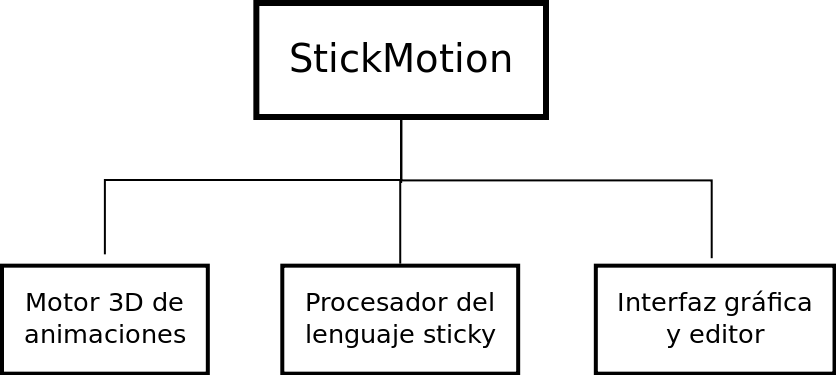
\includegraphics[width=0.9\textwidth]{./imagenes/descFuncional}\label{descFuncional}
   \caption{Esquema de la descomposición en distintos bloques funcionales.}
\end{center} \end{figure}

En la figura \ref{descFuncional} se muestra un esquema de la descomposición funcional que se llevará a cabo. Los distintos bloques se 
describirán a continuación. \\

   \subsection*{Motor 3D de animaciones}
   Este bloque será el encargado de llevar a cabo la creación y gestión de la escena 3D, siendo el responsable del renderizado del 
   \textbf{\textit{Stickman}} que se deberá mostrar en la interfaz, así como realizar y almacenar las animaciones que se deberán realizar
   definidas por el lenguaje. \\

   Deberá por tanto ofrecer una interfaz con funciones necesarias para la inclusión de animaciones en el Stickman, y obtener como salida
   una escena 3D que pueda ser mostrada en la interfaz gráfica. \\

   \subsection*{Procesador del lenguaje Sticky}
   Este bloque funcional será el cerebro de la interpretación del lenguaje Sticky diseñado, implementará las gramáticas empleando la librería
   ANTLR, y lo hará en base al lenguaje que se ha diseñado para tal efecto, al cual se le ha denominado \textbf{\textit{``Sticky''}}.\\

   Deberá por tanto recibir el código introducido por el usuario y emplearlo procesando las acciones pertinentes para comunicarse con el 
   motor 3D de animaciones en la realización de los movimientos que se especifiquen en el código \textbf{\textit{Sticky}}. \\


   \section{Requisitos funcionales}
   A continuación se enumerarán una serie de requisitos especificando las funciones que deberán realizar cada uno de los componentes en los
   que se ha dividido el diseño de la aplicación. \\

      \subsection{Motor 3D de animaciones}
      \begin{itemize}
         \item \textbf{RF1:} Deberá ofrecer la creación de una escena 3D que contenga la figura del Stickman.
         \item \textbf{RF2:} La figura Stickman deberá poseer 4 extremidades y 1 cabeza que podrán rotarse en cualquier dirección del 
               espacio tridimensional.
               \begin{itemize}
                  \item \textbf{RF2.1:} La rotación se realizará indicando el azimut y la elevación, en radianes, que se desea llevar a cabo,
                        y el tiempo, en milisegundos, que durará la misma.
               \end{itemize}
         \item \textbf{RF3:} El sistema debe permitir la rotación de la figura \textbf{\textit{Stickman}}.
               \begin{itemize}
                  \item \textbf{RF3.1:} La rotación se realizará indicando el azimut y la elevación, en radianes, que se desea llevar a
                        cabo, y el tiempo, en milisegundos, que durará la misma.
               \end{itemize}
         \item \textbf{RF4:} El sistema debe permitir la traslación de la figura \textbf{\textit{Stickman}}.
               \begin{itemize}
                  \item \textbf{RF4.1:} La traslación se realizará indicando el desplazamiento en \textit{X, Y} y \textit{Z}, siendo la unidad
                     la medida del antebrazo del \textbf{\textit{Stickman}}, y el tiempo en milisegundos que durará la misma.
               \end{itemize}
         \item \textbf{RF5:} Cada una de las 4 extremidades del Stickman poseerá un punto de flexión sobre el cual podrá doblarse.
               \begin{itemize}
                  \item \textbf{RF5.1:} La flexión se realizará indicando un ángulo en radianes y el tiempo en segundos que durará la misma.
               \end{itemize}
         \item \textbf{RF6:} La animación debe ser temporal, por lo que se debe almacenar el tiempo de animación actual.
               \begin{itemize}
                  \item \textbf{RF6.1:} El sistema debe facilitar el tiempo actual de animación cuando el usuario lo desee.
                  \item \textbf{RF6.2:} El sistema debe permitir la modificación del tiempo actual de animación cuando el usuario lo desee.
               \end{itemize}
         \end{itemize}

      \subsection{Procesador del lenguaje Sticky}
      \begin{itemize}
         \item \textbf{RF6:} Se seguirán las construcciones gramaticales, control de flujo y operaciones especificadas por la descripción
               del lenguaje \textbf{\textit{Sticky}}.
         \item \textbf{RF7:} Se ofrecerá una salida amigable en cuanto al reporte de errores, permitiendo en lo posible, la recuperación
               tras los mismos para continuar evaluando el resto del código.
         \item \textbf{RF8:} Para facilitar la depuración, se ofrecerá un nivel regulable de detalle de la salida esperada, de forma que
               se muestren distintos mensajes de depuración o \textit{``DEBUG''} si el usuario desea un mayor detalle sobre las operaciones
               que el procesador está realizando.
      \end{itemize}

      \subsection{Interfaz gráfica y editor}
      \begin{itemize}
         \item \textbf{RF9:} El sistema debe permitir la creación de nuevos documentos con código \textbf{\textit{Sticky}}.
         \item \textbf{RF10:} El sistema debe permitir la carga de archivos de código Sticky (extensión .stk) en la interfaz del editor.
         \item \textbf{RF11:} El sistema debe permitir almacenar el código Sticky insertado en el editor en un archivo en disco.
         \item \textbf{RF12:} El sistema debe permitir deshacer cambios sobre el código en el editor.
         \item \textbf{RF13:} El sistema debe permitir rehacer cambios sobre el código en el editor.
         \item \textbf{RF14:} El sistema debe permitir copiar, cortar y pegar porciones de código en el editor.
         \item \textbf{RF15:} El sistema debe permitir iniciar la interpretación del código contenido en el editor.
         \item \textbf{RF16:} El sistema debe permitir detener una interpretación en curso.
         \item \textbf{RF17:} El sistema debe permitir limpiar el editor de código.
         \item \textbf{RF18:} El sistema debe generar código cuando el usuario lo desee. El código que debe poder generar son el condicional
               \textit{``si``} y los bucles \textit{''mientras``} y \textit{''para``}.
         \item \textbf{RF19:} El sistema debe permitir editar el código Sticky por teclado desde la propia interfaz del editor.
         \item \textbf{RF20:} La interfaz debe mostrar mostrar la escena 3D del Stickman en animación.
         \item \textbf{RF21:} El sistema debe permitir, en el editor, resaltar la sintaxis propia del lenguaje \textbf{\textit{Sticky}}.
      \end{itemize}

   
   \section{Requisitos no funcionales}
   Para poder llevar a cabo todos los objetivos correctamente nuestra aplicación deberá cumplir con la siguiente serie de requisitos no funcionales:
   \begin{itemize}
      \item \textbf{RNF1:} El programa deberá ser desarrollado en Java, siguiendo el programa de la asignatura, y ofreciendo además
            portabilidad en cuanto a plataforma de ejecución.
      \item \textbf{RNF2:} El procesamiento del lenguaje deberá realizarse empleando la librería ANTLR para la creación de reconocedores de lenguaje.
      \item \textbf{RNF3:} La aplicación deberá ofrecer un manejo intuitivo y sencillo.
   \end{itemize}
